\documentclass[11pt]{article}

\usepackage[margin=0.88in]{geometry}
\usepackage[T1]{fontenc}
\usepackage{amsmath,amssymb,amsthm,bm}
\usepackage{booktabs}
\usepackage{graphicx}
\usepackage{microtype}
\usepackage[numbers,sort&compress]{natbib}
\usepackage[colorlinks=true,allcolors=blue]{hyperref}

\newtheorem{theorem}{Theorem}
\newtheorem{proposition}{Proposition}
\newtheorem{remark}{Remark}
\newcommand{\J}{\mathbf{J}}
\newcommand{\Q}{\mathbf{Q}}
\newcommand{\I}{\mathbf{I}}
\newcommand{\E}{\mathbb{E}}
\newcommand{\R}{\mathbb{R}}
\newcommand{\norm}[1]{\left\lVert #1\right\rVert}
\newcommand{\projector}{\Q\Q^{\mathsf T}}

\title{\textbf{Randomized Subspace QAOA:\\
Certified Active-Subspace Optimization for Multi-Angle QAOA}}
\author{Molena Huynh\\
North Carolina State University\\
\texttt{molena.huynh@jmp.com}}
\date{July 14, 2026}

\begin{document}
\maketitle

\begin{abstract}
Multi-angle QAOA (ma-QAOA) assigns an independent parameter to every mixer and
cost term, increasing the depth-$p$ parameter dimension to
$d=p(|E|+|V|)$.  We introduce Randomized Subspace QAOA (RSQ), which optimizes
inside a matrix-free active subspace of the Jacobian of the per-edge observable
vector.  RSQ accesses the Jacobian only through Jacobian--vector and
vector--Jacobian products, selects rank with a randomized residual certificate,
checks that certificate during optimization, and updates a recycled basis by
augmenting and recompressing it.  A separate forward-only variant replaces every
reverse product, including the refresh certificate, by finite-difference
directional probes.  We prove that the scalar ma-QAOA gradient lies in the
Jacobian row space and bound the first-order objective change discarded by a
certified subspace.  On a released CPU benchmark of 36 paired MaxCut instances
(three graph families, $n\in\{8,10\}$, $p\in\{1,2\}$, and three seeds),
two-sided RSQ at tolerance $10^{-2}$ reduces the optimized dimension by $41.5\%$
at $p=1$ while changing approximation ratio by $-0.21\pm0.89$ percentage points
(mean $\pm$ two standard errors) relative to full ma-QAOA.  At $p=2$ it reduces
the dimension by $70.8\%$ with a $-2.86\pm1.43$ point change.  The forward-only
variant is more compressed but loses more quality.  Instrumented operator counts
also show that subspace discovery has substantial setup cost on these small
simulators; we therefore claim controlled parameter compression, not a quantum
query advantage.  The results identify both a useful shallow-depth regime and a
failure boundary that any larger-scale RSQ claim must cross.
\end{abstract}

\section{Introduction}

The Quantum Approximate Optimization Algorithm (QAOA) alternates a cost
Hamiltonian and a mixer, then adjusts their angles with a classical optimizer
\citep{farhi2014qaoa,hadfield2019quantum,zhou2020qaoa}.  Multi-angle QAOA
(ma-QAOA) replaces the two shared angles in each layer by one phase parameter per
cost term and one mixer parameter per qubit \citep{herrman2022multiangle}.  This
removes a strong tying constraint, but it changes the classical search dimension
from $2p$ to
\begin{equation}
 d=p(|E|+|V|).
 \label{eq:dimension}
\end{equation}
The added coordinates are useful only when they create independent changes in
measurable observables.  Searching all of them indiscriminately can therefore
spend optimization effort in directions to which the circuit is locally
insensitive.

Existing reductions approach this proliferation from three directions.
Symmetry-based reductions tie angles that graph automorphisms make equivalent
\citep{shi2022notallangles}; they are exact but compress only as far as the
automorphism group allows, and many random graphs have trivial symmetry.
Measurement-compression and landscape-reconstruction methods exploit low-rank
structure in what is measured or in the landscape itself
\citep{he2026hgle,jain2024lowrank}, but they do not by themselves produce a
reduced \emph{search space} equipped with a quantitative acceptance test.
Active-subspace methods \citep{constantine2014active,constantine2015active}
seek the directions along which a function is locally most sensitive and
optimize only there; they are the natural template for ma-QAOA, whose added
coordinates are useful exactly when they move measurable observables.  The
obstacle is practical.  Explicitly forming the Jacobian that defines the
active subspace costs more than the search it is meant to save, and a subspace
fixed once at initialization has no way to notice that it has gone stale as
the optimizer moves.  What is missing is a construction that touches the
Jacobian only through operator actions, reports a computable certificate of
the sensitivity it discards, and refreshes itself when that certificate fails.
RSQ is that construction.

RSQ combines an observable-space formulation with adaptive matrix-free
randomized linear algebra.  The numerical primitive is fixed-tolerance
randomized QB, which approximates a linear operator through products, estimates
its residual from random probes, and chooses its output rank adaptively
\citep{halko2011finding,yu2018randqb,martinsson2020randomized}.
Our contribution is not a new general-purpose QB factorization.  It is the
quantum-optimization construction around that primitive: the operator is a
ma-QAOA sensitivity map; its right singular space becomes the feasible search
space; its estimated residual becomes a refresh criterion; and a forward-only
diagnostic makes the restricted variant operational without an adjoint.  The
experiments then count the setup cost that this construction introduces instead
of treating dimension reduction as a proxy for resource savings.

The central empirical question is not whether a subspace can be constructed,
but whether the resulting compression preserves optimization quality after its
setup cost is counted.  We answer that question on a deliberately small,
fully released benchmark.  The answer is conditional: at depth one, RSQ closely
tracks full ma-QAOA while optimizing substantially fewer coordinates; at depth
two, stronger compression incurs a measurable quality loss; and on the studied
simulator the operator setup is more expensive than direct optimization.  This
claim boundary is a result, because it separates structural compression from an
unsubstantiated hardware-speedup claim.

\paragraph{Contributions.}
\begin{enumerate}
\item We formulate the per-edge observable Jacobian as a matrix-free operator
and prove that its row space contains the local gradient of any weighted
MaxCut objective.
\item We give a certificate-gated optimizer with a recycled update that can
rotate a saturated basis: old directions are augmented by current residual
directions and the combined space is recompressed.
\item We give a genuinely forward-only build and refresh path.  A dedicated
test requires zero vector--Jacobian products throughout this path.
\item We release paired results, operator counters, tests, figures, and the
script that regenerates every aggregate in this article.
\end{enumerate}

\section{Observable-space formulation}
\label{sec:formulation}

Let $G=(V,E)$ be an unweighted graph and let
$C_e=(I-Z_iZ_j)/2$ for $e=(i,j)$.  A depth-$p$ ma-QAOA state is
\begin{equation}
 |\psi(\bm\theta)\rangle=
 \prod_{\ell=1}^{p}
 \left[\prod_{i\in V}e^{-i\beta_{\ell i}X_i}
 \prod_{e\in E}e^{-i\gamma_{\ell e}C_e}\right]
 |+\rangle^{\otimes |V|}.
 \label{eq:state}
\end{equation}
Define the vector of local observables
\begin{equation}
 F(\bm\theta)=
 \big(\langle\psi(\bm\theta)|C_e|\psi(\bm\theta)\rangle\big)_{e\in E}
 \in\R^{m}, \qquad m=|E|,
\end{equation}
and its Jacobian
\begin{equation}
 \J(\bm\theta)=\frac{\partial F}{\partial\bm\theta}
 \in\R^{m\times d}.
 \label{eq:jacobian}
\end{equation}
For edge weights $w\in\R^m$, the expected cut is
$C(\bm\theta)=w^{\mathsf T}F(\bm\theta)$.

\begin{proposition}[The local objective gradient is active]
\label{prop:gradient}
At every differentiable point,
\begin{equation}
 \nabla C(\bm\theta)=\J(\bm\theta)^{\mathsf T}w
 \in \operatorname{range}(\J(\bm\theta)^{\mathsf T}).
\end{equation}
Consequently, the steepest first-order change of any weighted sum of the chosen
observables lies in the parameter-space row span of $\J$.
\end{proposition}
\begin{proof}
Apply the chain rule to $C=w^{\mathsf T}F$.
\end{proof}

This statement is local.  The row space may rotate as optimization moves, which
is why a fixed subspace can fail even if it is exact at its construction point.
It also gives an algebraic ceiling
\begin{equation}
 \operatorname{rank}(\J)\leq \min(m,d).
 \label{eq:rankceiling}
\end{equation}
For the observable choice used here, $m$ does not grow with QAOA depth while
$d=p(m+n)$ does.  Depth can therefore increase the compressible complement even
without additional numerical singular-value decay.

\section{Randomized Subspace QAOA}
\label{sec:method}

\subsection{Matrix-free sensitivity actions}

At an anchor $\bm\theta_0$, RSQ exposes two actions without materializing
$\J$:
\begin{align}
 \operatorname{jvp}(v)&=\J(\bm\theta_0)v,\\
 \operatorname{vjp}(u)&=\J(\bm\theta_0)^{\mathsf T}u.
\end{align}
The implementation evaluates the VJP by reverse-mode automatic differentiation.
It evaluates a JVP either by automatic differentiation or by the central
finite difference
\begin{equation}
 \J v = \frac{F(\bm\theta_0+h v)-F(\bm\theta_0-h v)}{2h}+O(h^2),
 \label{eq:fd}
\end{equation}
with $h=10^{-4}$.  The released tests compare both actions to a dense Jacobian
and verify the adjoint identity.

\subsection{Adaptive basis and residual certificate}

RSQ factors $A=\J^{\mathsf T}$ as $A\approx \Q B$, where
$\Q\in\R^{d\times r}$ has orthonormal columns and
$B=\Q^{\mathsf T}A$.  Randomized QB expands $\Q$ in blocks until an estimated
relative residual falls below $\varepsilon$.  We expose a Frobenius certificate
and a power-iteration spectral certificate, following established randomized
matrix-free approximation \citep{halko2011finding,yu2018randqb,musco2015randomized}.  The optimization
variables are $z\in\R^r$ with
\begin{equation}
 \bm\theta=\bm\theta_0+\Q z.
 \label{eq:reduced}
\end{equation}

Every $K=25$ steps, RSQ evaluates the residual at the current point.  If the
relative residual exceeds $\varepsilon_{\mathrm{refresh}}=0.05$, it reanchors.
A naive recycled implementation can freeze: if the old basis already has the
maximum requested rank, no new column can enter even when the residual is
large.  Our update instead permits a temporary augmented basis, adds current
residual directions, and takes the singular value decomposition of the small
coefficient matrix $B$.  Rotating by its leading left singular vectors returns
the best requested-rank basis available in the augmented space.  This step is
both implemented and regression tested.

\subsection{Forward-only build and refresh}

The forward-only variant selects an $r$-dimensional trial space by applying JVPs
to a Gaussian parameter sketch and solving the resulting small Rayleigh--Ritz
problem.  Its refresh certificate also uses only JVPs.  For independent
$v_i\sim\mathcal N(0,I_d)$, define
\begin{equation}
 \widehat\rho_F^2=
 \frac{\sum_{i=1}^{s}\norm{\J(\I-\projector)v_i}^2}
      {\sum_{i=1}^{s}\norm{\J v_i}^2}.
 \label{eq:forwardcertificate}
\end{equation}
Both numerator terms are evaluated with forward differences.  The identity
$\E\norm{Mv}^2=\norm{M}_F^2$ implies that the numerator and denominator
converge to the corresponding squared Frobenius norms as $s$ grows.  We use
$s=12$.  Unlike a spectral certificate, Eq.~\eqref{eq:forwardcertificate}
controls average discarded sensitivity; a missed worst direction remains a
failure mode.

\begin{proposition}[Moment identity for the forward residual diagnostic]
\label{prop:residual-moments}
Let $R=\J(\I-P)$ and let $v_1,\ldots,v_s$ be independent standard Gaussian
vectors.  For
\begin{equation}
 \widehat a_s=\frac{1}{s}\sum_{i=1}^{s}\norm{Rv_i}^{2},
\end{equation}
we have
\begin{equation}
 \E[\widehat a_s]=\norm{R}_F^2,
 \qquad
 \operatorname{Var}(\widehat a_s)
 =\frac{2}{s}\norm{R^{\mathsf T}R}_F^2.
 \label{eq:residual-moments}
\end{equation}
The analogous identities hold for the denominator of
Eq.~\eqref{eq:forwardcertificate} with $R$ replaced by $\J$.
\end{proposition}
\begin{proof}
Write $\norm{Rv_i}^2=v_i^{\mathsf T}R^{\mathsf T}Rv_i$ and apply the first two
moments of a real Gaussian quadratic form.  Averaging independent probes divides
the variance by $s$.
\end{proof}

Proposition~\ref{prop:residual-moments} justifies the diagnostic as a consistent
randomized estimator.  It does not make the ratio of its numerator and
denominator unbiased, nor does a finite probe count provide a deterministic
upper bound.  Accordingly, the implementation uses the observed ratio as a
refresh trigger, while Theorem~\ref{thm:loss} below is conditional on the true
operator residual.  This distinction is important when interpreting the word
``certified'' in a finite randomized run.

\subsection{First-order truncation bound}

\begin{theorem}[Certified local objective loss]
\label{thm:loss}
Let $P=\projector$ and suppose
$\norm{\J(\bm\theta)(I-P)}_2\leq\varepsilon$.  If $F$ is twice continuously
differentiable in a neighborhood of $\bm\theta$, then for a step $\Delta$,
\begin{equation}
 \left|C(\bm\theta+\Delta)-C(\bm\theta+P\Delta)\right|
 \leq \norm{w}\,\varepsilon\norm{\Delta}+O(\norm{\Delta}^2).
 \label{eq:lossbound}
\end{equation}
\end{theorem}
\begin{proof}
Taylor expansion gives
$F(\bm\theta+\Delta)-F(\bm\theta+P\Delta)
=\J(\bm\theta)(I-P)\Delta+O(\norm{\Delta}^2)$.
Apply the operator-norm bound and then Cauchy--Schwarz to
$w^{\mathsf T}[F(\bm\theta+\Delta)-F(\bm\theta+P\Delta)]$.
\end{proof}

The theorem does not give global convergence or an approximation-ratio
guarantee.  It states exactly what the residual certificate controls: the
first-order change discarded at the current anchor.

\paragraph{Algorithm.}
The implemented loop is:
\begin{enumerate}
\item construct $\Q$ at $\bm\theta_0$ to tolerance $\varepsilon$;
\item run one Adam step in $z$ for the objective
$-C(\bm\theta_0+\Q z)$;
\item every $K$ steps, evaluate the current residual;
\item when it exceeds threshold, reanchor, augment and recompress the recycled
basis, reset $z$, and continue.
\end{enumerate}
All forward evaluations, JVPs, VJPs, ranks, and refreshes are instrumented.

\section{Experimental protocol}
\label{sec:experiments}

We test unweighted MaxCut on three graph families: random 3-regular graphs,
Erdos--Renyi graphs with edge probability $0.5$, and rings.  The grid contains
$n\in\{8,10\}$, $p\in\{1,2\}$, and seeds $\{0,1,2\}$: 36 paired instances.
The simulator is a pure-PyTorch, complex-128 statevector implementation
\citep{paszke2019pytorch}; an optional PennyLane backend supplies an independent
cross-check \citep{bergholm2018pennylane}.  Brute-force MaxCut gives the exact
denominator for the approximation ratio.

Every optimizer receives 100 Adam steps.  Full ma-QAOA, fixed-rank RSQ, and
two-sided RSQ share the same instance-specific initial angle vector.  The
symmetry baseline uses the same seed in its reduced parameterization.  We
compare:
\begin{itemize}
\item full ma-QAOA;
\item angles tied by graph-automorphism orbits;
\item a rank-8 dense-SVD oracle fixed at the initial Jacobian (its Jacobian setup
cost is excluded, so this is an oracle rather than a deployable baseline);
\item two-sided adaptive RSQ at $\varepsilon\in\{10^{-1},10^{-2}\}$;
\item forward-only rank-8 RSQ.
\end{itemize}
The primary outcome is expected-cut approximation ratio.  Parameter count is
the dimension optimized after construction.  Paired differences subtract the
full ma-QAOA ratio on the same graph and seed.  We report mean and standard
deviation for raw ratios and mean $\pm$ two standard errors for paired changes.
No hypothesis test is used to turn absence of significance into equivalence.

\section{Results}
\label{sec:results}

\subsection{Depth one: compression with a small paired change}

At $p=1$, full ma-QAOA optimizes $22.4$ parameters on average and attains
$0.851\pm0.053$.  RSQ at $\varepsilon=10^{-2}$ optimizes $13.4$ parameters, a
$41.5\%$ reduction, and attains $0.849\pm0.053$.  The paired change is
$-0.21\pm0.89$ percentage points.  This interval includes zero, but the
experiment was not designed as a formal equivalence trial; the correct
interpretation is that no material average gap is resolved at the precision of
this released grid.

The rank-8 fixed-subspace oracle reaches only $0.756\pm0.047$, a paired change of
$-9.54\pm2.18$ points.  Forward-only rank-8 RSQ reaches
$0.819\pm0.049$, improving substantially on the fixed oracle but remaining
$3.18\pm1.43$ points below full ma-QAOA.  Adaptive refresh is therefore useful,
but forward-only access does not close the depth-one quality gap at rank 8.

\begin{figure}[t]
\centering
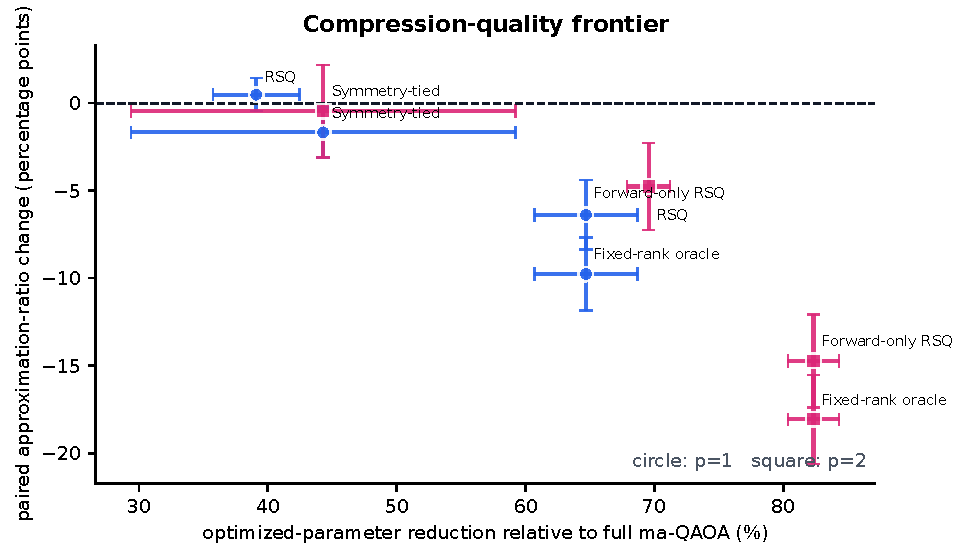
\includegraphics[width=0.96\linewidth]{figures/figure1_tradeoff.pdf}
\caption{Compression--quality frontier.  Horizontal coordinates are optimized
parameter reduction relative to full ma-QAOA.  Vertical coordinates are paired
approximation-ratio changes; error bars show two standard errors.  The main RSQ
point at $p=1$ approaches the zero-change line, whereas stronger compression and
depth two expose a larger quality cost.}
\label{fig:tradeoff}
\end{figure}

\subsection{Depth two: the failure boundary becomes visible}

At $p=2$, full ma-QAOA optimizes $44.9$ parameters on average and attains
$0.925\pm0.057$.  RSQ optimizes the same $13.4$-dimensional observable-controlled
subspace as at depth one, now a $70.8\%$ reduction.  At tolerance $10^{-2}$ its
ratio is $0.896\pm0.060$, a paired change of $-2.86\pm1.43$ points.  The added
layer grows the ambient parameter space without growing the observable count,
but the more aggressive compression no longer preserves the full optimizer's
quality.

The forward-only rank-8 variant loses $9.62\pm2.02$ points at depth two.  The
fixed rank-8 oracle loses $16.55\pm1.87$ points.  These results rule out a blanket
claim that a very small initial sensitivity space is sufficient for ma-QAOA.
The subspace must be large enough, must be refreshed, and may need richer
observables at higher depth.

\begin{figure}[t]
\centering

\includegraphics[width=0.90\linewidth]{figures/figure2_family.pdf}
\caption{Paired quality change for RSQ at $\varepsilon=0.1$, separated by graph
family.  Bars show means and error bars show two standard errors.  The
depth-two loss is present across all three tested families; wide intervals on
some families reflect the small released grid.}
\label{fig:family}
\end{figure}

\subsection{The certificate identifies algebraic, not extra numerical, rank}

Across the tested tolerances, two-sided RSQ retains $13.4$ directions on average,
the average number of edge observables.  Tightening the tolerance from $0.1$ to
$0.01$ does not materially change the rank or the quality.  Thus this benchmark
does not show additional numerical low-rank decay beyond the algebraic ceiling
in Eq.~\eqref{eq:rankceiling}.  What grows with depth is the complement between
$m$ and $d$, not a newly discovered decay of the nonzero spectrum.

\begin{figure}[t]
\centering
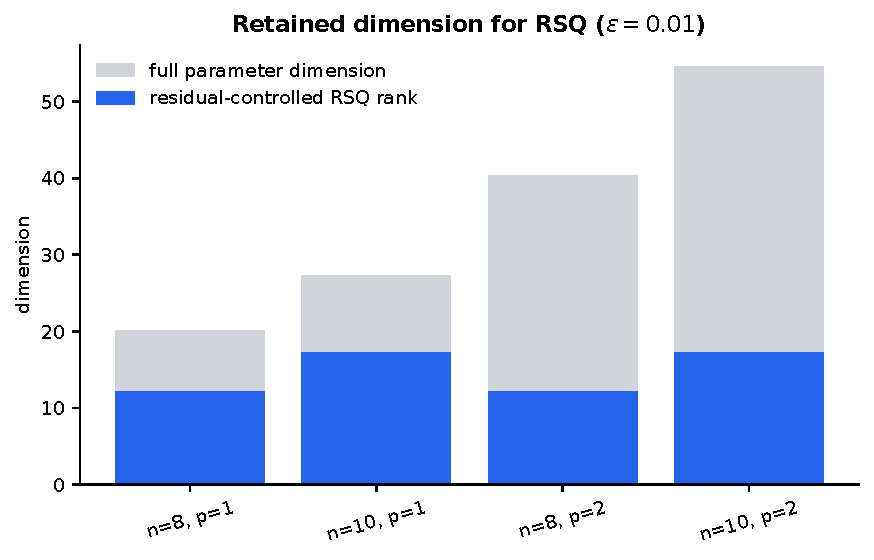
\includegraphics[width=0.90\linewidth]{figures/figure4_rank.pdf}
\caption{Ambient ma-QAOA dimension and certified RSQ rank, averaged across graph
families and seeds.  The observable count controls the retained dimension while
the ambient parameter count doubles with depth.}
\label{fig:rank}
\end{figure}

\subsection{Setup cost prevents a query-efficiency claim}

At tolerance $0.1$, the two-sided method averages 237 forward-$F$ evaluations, 119 JVPs, and 358
VJPs at $p=1$, compared with 100 forward evaluations and 100 VJPs for the full
baseline under the simulator's accounting.  At $p=2$ the corresponding RSQ
counts increase to 267, 134, and 408.  The forward-only path uses no VJP, as
intended, but requires about 285--288 forward evaluations and 143--144 JVPs.
These categories are instrumentation counters, not additive physical-shot
counts; a JVP by central difference contains forward evaluations already
recorded by the lower-level counter.

\begin{figure}[t]
\centering

\includegraphics[width=0.92\linewidth]{figures/figure3_operator_budget.pdf}
\caption{Mean instrumented operator counts.  Categories are shown separately
and are not additive.  On these small exact simulators, subspace discovery and
refresh cost more operator applications than direct full-space optimization.}
\label{fig:budget}
\end{figure}

\begin{table}[t]
\centering
\caption{Released 36-instance benchmark.  Approximation ratios are mean
$\pm$ standard deviation.  Paired changes are relative to full ma-QAOA on the
same instance and are mean $\pm$ two standard errors in percentage points.}
\label{tab:summary}
\resizebox{\textwidth}{!}{\begin{tabular}{lrrrr}
\toprule
Method & Depth & Parameters & Approx. ratio & Paired change \\
\midrule
Full ma-QAOA & 1 & 23.7 & 0.862 $\pm$ 0.053 & -- \\
Symmetry-tied & 1 & 14.4 & 0.845 $\pm$ 0.065 & -1.67 $\pm$ 1.42 pp \\
Fixed-rank oracle & 1 & 8.0 & 0.764 $\pm$ 0.051 & -9.77 $\pm$ 2.09 pp \\
RSQ ($\varepsilon=0.01$) & 1 & 14.7 & 0.867 $\pm$ 0.051 & +0.48 $\pm$ 0.94 pp \\
RSQ ($\varepsilon=0.1$) & 1 & 14.7 & 0.862 $\pm$ 0.051 & -0.03 $\pm$ 0.79 pp \\
Forward-only RSQ & 1 & 8.0 & 0.798 $\pm$ 0.055 & -6.39 $\pm$ 1.98 pp \\
\addlinespace
Full ma-QAOA & 2 & 47.4 & 0.945 $\pm$ 0.044 & -- \\
Symmetry-tied & 2 & 28.7 & 0.940 $\pm$ 0.064 & -0.45 $\pm$ 2.64 pp \\
Fixed-rank oracle & 2 & 8.0 & 0.764 $\pm$ 0.048 & -18.07 $\pm$ 2.54 pp \\
RSQ ($\varepsilon=0.01$) & 2 & 14.7 & 0.897 $\pm$ 0.054 & -4.77 $\pm$ 2.47 pp \\
RSQ ($\varepsilon=0.1$) & 2 & 14.7 & 0.906 $\pm$ 0.058 & -3.88 $\pm$ 1.84 pp \\
Forward-only RSQ & 2 & 8.0 & 0.797 $\pm$ 0.053 & -14.73 $\pm$ 2.65 pp \\
\bottomrule
\end{tabular}
}
\end{table}

\section{Discussion}

The experiments support a narrower and more useful conclusion than the original
resource-efficiency hypothesis.  At depth one, the observable row space removes
roughly two fifths of the optimized coordinates with little resolved change in
mean quality.  At depth two, the same observable dimension removes roughly seven
tenths of the coordinates but loses about three approximation-ratio points.
Parameter compression is therefore real, while quality preservation is
depth-dependent.

The comparison to the fixed-rank oracle clarifies why refresh matters.  Even an
initial dense SVD is poor when frozen.  The relevant object is a moving local row
space, not a universal low-dimensional parameterization.  The repaired recycled
update is essential here: simply seeding a saturated QB factorization with the
old basis prevents rotation and produced a large artificial quality gap in an
earlier implementation.  The regression suite now checks the corrected update.

The forward-only path establishes feasibility but not parity.  It avoids every
VJP, including during refresh, and outperforms the equally sized fixed oracle.
Its remaining quality loss can arise from restricting the Rayleigh--Ritz search
to a random trial space, finite-difference error, and the use of an average
Frobenius drift certificate.  Hardware studies should compare larger sketches,
common-random-number shot estimators, and worst-direction forward certificates.

Most importantly, fewer optimized coordinates do not automatically mean fewer
quantum queries.  The released small-instance counts go in the opposite
direction because basis construction is expensive.  A genuine query advantage
would require amortizing a basis across related instances, using hardware-native
batching, or reaching a scale at which full-gradient cost grows faster than the
matrix-free sketch.  Those are testable future conditions, not conclusions of
the present data.

\section{Limitations}

The benchmark contains only 36 paired instances, $n\leq10$, depths one and two,
and exact statevector objectives.  It does not model shot noise, device noise,
compilation, queue latency, or weighted spin glasses.  The graph families are
standard but narrow.  One hundred optimizer steps may favor some parameterizations
over others, and no hyperparameter sweep is used to optimize each baseline
separately.  The fixed-rank oracle excludes its dense-Jacobian setup cost and is
therefore only a quality reference.  The randomized residual ratios are finite-
probe estimators and can underestimate the true residual; no deterministic or
run-wise coverage guarantee is claimed for the chosen probe count.  Finally,
the observable vector contains
per-edge costs; adding mixer observables, commutators, or layer-resolved features
could raise rank but improve high-depth fidelity.

\section{Reproducibility}

The canonical package is the repository's \texttt{code/} directory.  A clean
environment can install and verify it with
\begin{verbatim}
python -m pip install -e 'code[dev,experiments]'
python -m pytest code/tests -q
cd code
python experiments/run_experiment.py \
  --config experiments/configs/maxcut_small.yaml
python experiments/summarize_results.py
\end{verbatim}
The experiment runner writes one CSV row per method, instance, and seed.  The
summarizer reads only that CSV and regenerates the four figures, Table
\ref{tab:summary}, and a machine-readable JSON summary.  Tests cover the
statevector against a dense reference, JVP/VJP consistency, fixed-tolerance
factorization, spectral residual estimation, basis recycling, the forward-only
zero-VJP invariant, baselines, and the optional PennyLane cross-check.

\section{Conclusion}

RSQ turns the local observable Jacobian of ma-QAOA into an adaptive optimization
space without forming the Jacobian.  Its certificate has a precise role: it
bounds discarded first-order sensitivity and decides when the space must be
updated.  On the released benchmark, this mechanism preserves depth-one quality
under substantial parameter compression, reveals a depth-two compression--quality
tradeoff, and carries nontrivial setup cost.  These findings establish a
fact-checkable baseline for future randomized-subspace quantum optimization and
define the evidence required before stronger query-efficiency claims are made.

\bibliographystyle{plainnat}
\bibliography{refs}

\end{document}
